\documentclass[11pt]{article}
%\usepackage{fullpage,graphicx,algorithm,algorithmic,bm,amsmath,amsthm,amssymb,color,hyperref,cite,natbib}

% if you need to pass options to natbib, use, e.g.:
%\PassOptionsToPackage{numbers}{natbib}
\usepackage{natbib,fullpage}
\usepackage{bm,amsmath,amsthm,amssymb,multicol,algorithmic,algorithm,enumitem}
\usepackage{wrapfig,lipsum}
\usepackage[textwidth=1cm,textsize=footnotesize]{todonotes}

% ready for submission
\usepackage{neurips_2020}

\usepackage[colorlinks=true,
linkcolor=red,
urlcolor=blue,
citecolor=blue]{hyperref}
\usepackage{hyperref}
\usepackage{cleveref}
\usepackage{subfigure}

\setlength{\parskip}{.2cm}


\def\M{\mathcal{M}}
\def\A{\mathcal{A}}
\def\Z{\mathcal{Z}}
\def\S{\mathcal{S}}
\def\D{\mathcal{D}}
\def\R{\mathcal{R}}
\def\P{\mathcal{P}}
\def\K{\mathcal{K}}
\def\E{\mathbb{E}}
\def\F{\mathfrak{F}}
\def\l{\boldsymbol{\ell}}

\newtheorem{Fact}{Fact}
\newtheorem{Lemma}{Lemma}
\newtheorem{Prop}{Proposition}
\newtheorem{Theorem}{Theorem} 
\newtheorem{Def}{Definition}
\newtheorem{Corollary}{Corollary}
\newtheorem{Conjecture}{Conjecture}
\newtheorem{Property}{Property}
\newtheorem{Observation}{Observation}
%\theorembodyfont{\rmfamily}
\newtheorem{Exa}{Example}
\newtheorem{assumption}{H\!\!}
\newtheorem{assumptionA}{S\!\!}
\newtheorem{assumptionL}{L\!\!}
\newtheorem{Remark}{Remark}
\newtheorem*{Lemma*}{Lemma}
\newtheorem*{Theorem*}{Theorem}
 \makeatletter
\renewenvironment{proof}[1][\proofname]{%
   \par\pushQED{\qed}\normalfont%
   \topsep6\p@\@plus6\p@\relax
   \trivlist\item[\hskip\labelsep\bfseries#1]%
   \ignorespaces
}{%
   \popQED\endtrivlist\@endpefalse
}
\makeatother

%%%%%%%%%%% Stuffs for Tikz %%%%%%%%%%%%%%%%%%
\usepackage{pgfplots}
\usepackage{xargs}
\usepackage{stmaryrd}
\usetikzlibrary{arrows,shapes,calc,tikzmark,backgrounds,matrix,decorations.markings}
\usepgfplotslibrary{fillbetween}

\pgfplotsset{compat=1.3}

\usepackage{relsize}
\tikzset{fontscale/.style = {font=\relsize{#1}}
    }

\definecolor{lavander}{cmyk}{0,0.48,0,0}
\definecolor{violet}{cmyk}{0.79,0.88,0,0}
\definecolor{burntorange}{cmyk}{0,0.52,1,0}

\def\lav{lavander!90}
\def\oran{orange!30}

\definecolor{asuorange}{rgb}{1,0.699,0.0625}
\definecolor{asured}{rgb}{0.598,0,0.199}
\definecolor{asuborder}{rgb}{0.953,0.484,0}
\definecolor{asugrey}{rgb}{0.309,0.332,0.340}
\definecolor{asublue}{rgb}{0,0.555,0.836}
\definecolor{asugold}{rgb}{1,0.777,0.008}

%%%%%%%%%%%%%%%%%%%%%%%%%%%%%%%%%%%%%


\usepackage{shortcuts_OPT}

%\renewcommand{\textwidth}{5.5in}

% Here's the definition of Sb, stolen from amstex
    \makeatletter
    \def\multilimits@{\bgroup
  \Let@
  \restore@math@cr
  \default@tag
 \baselineskip\fontdimen10 \scriptfont\tw@
 \advance\baselineskip\fontdimen12 \scriptfont\tw@
 \lineskip\thr@@\fontdimen8 \scriptfont\thr@@
 \lineskiplimit\lineskip
 \vbox\bgroup\ialign\bgroup\hfil$\m@th\scriptstyle{##}$\hfil\crcr}
    \def\Sb{_\multilimits@}
    \def\endSb{\crcr\egroup\egroup\egroup}
\makeatother

\newtheoremstyle{k}         %name
    {\baselineskip}{2\topsep}      %space above and below
    {\rm}                   %Body font
    {0pt}{\bfseries}  %Heading indent and font
    {}                      %after heading
    { }                      %head after space
    {\thmname{#1}\thmnumber{#2}.}

\theoremstyle{k}
\newtheorem{q}{Q}
\parindent=0pt

%\newcommand{\eric}[1]{\todo[color=red!20]{{\bf EM:} #1}}
%\newcommand{\erici}[1]{\todo[color=red!20,inline]{{\bf EM:} #1}}
%\newcommand{\belhal}[1]{\todo[color=green!20]{{\bf BK:} #1}}
%\newcommand{\belhali}[1]{\todo[color=green!20,inline]{{\bf BK:} #1}}
%\newcommand{\toco}[1]{\todo[color=yellow!20]{{\bf To:} #1}}



\makeatletter
\DeclareRobustCommand*\cal{\@fontswitch\relax\mathcal}
\makeatother

\begin{document}
\title{Optimistic Acceleration for Adaptive Optimization}
%\author{}
\date{\today}

\maketitle


\section{Experiments}

In this section, we provide experiments on classification tasks with various neural network architectures and datasets to demonstrate the effectiveness of \textsc{OPTIMISTIC-AMSGrad} in practical applications.

\textbf{Methods.}\hspace{0.1in}We consider two baselines. The first one is the original \textsc{AMSGrad}. 
The hyper-parameters are set to be $\beta_1$ and $\beta_2$ to be $0.9$ and $0.999$ respectively, as recommended by \cite{RKK18}. We tune the learning rate $\eta$ over a fine grid and report the best result. 

The other competing method is the aforementioned
\textsc{Optimistic-Adam$+\hat{v}_t$} method (Algorithm \ref{OPT-DISZ}) as in Section 3. The key difference is that it uses previous gradient as the gradient prediction of the next iteration. We also report the best result achieved by tuning the step size $\eta$ for \textsc{Optimistic-Adam$+\hat{v}_t$}.


For \textsc{Optimistic-AMSGrad}, we use the same $\beta_1$, $\beta_2$ and 
the best step size $\eta$ of \textsc{AMSGrad} for a fair evaluation of the improvement brought by the extra optimistic step. Yet,
\textsc{Optimistic-AMSGrad} has an additional parameter $r$ that controls the number of previous gradients used for gradient prediction. Fortunately, we observe similar performance of \textsc{Optimistic-AMSGrad} with different values of $r$. Hence, we report $r=5$ for now when comparing with other baselines. We will address on the choice of $r$ at the end of this section.

In all experiments, all the optimization algorithms are initialized at the same point. We report the results averaged over 5 repetitions.

\textbf{Datasets.}\hspace{0.1in}Following \cite{RKK18} and \cite{KB15}, we compare different algorithms on \textit{MNIST}, \textit{CIFAR10},
\textit{CIFAR100}, and \textit{IMDB} datasets. 
For \textit{MNIST}, we use two noisy variants named as 1.65\textit{MNIST-back-rand} and 1.65\textit{MNIST-back-image} from \cite{MNIST07}. They both have 12000 training samples and 50000 test samples, where random background is inserted to the original \textit{MNIST} hand written 
digit images. For \textit{MNIST-back-rand}, each image is inserted with a random background, whose pixel values generated uniformly from 0 to 255, while \textit{MNIST-back-image} takes random patches from a black and white as noisy background.
The input dimension is 784 ($28\times 28$) and the number of classes is $10$. \textit{CIFAR10} and \textit{CIFAR100} are popular computer-vision datasets consisting of 50000 training images and 10000 test images, of size $32\times 32$. The number of classes are 10 and 100, respectively. The \textit{IMDB} movie review dataset is a binary classification dataset with 25000 training and testing samples respectively. It is a popular datasets for text classification.

\textbf{Network architecture.}\hspace{0.1in}We adopt a multi-layer fully-connected neural network with input layer followed by a hidden layer with $200$ nodes, which is connected to another layer with $100$ nodes before the output layer. The activation function is ReLU for hidden layers, and softmax for the output layer. This network is tested on \textit{MNIST} variants. Since convolutional networks are popular for image classification tasks, we consider an ALL-CNN architecture proposed by \cite{CNN15}, which is constructed with several convolutional blocks and dropout layers. In addition, we also apply residual networks, Resnet-18 and Resnet-50~\cite{Rnet16}, which have achieved many state-of-the-art results. For the texture \textit{IMDB} dataset, we consider training a Long-Short Term Memory (LSTM) network. The network includes a word embedding layer with 5000 input entries representing most frequent words in the dataset, and each word is embedded into a 32 dimensional space. The output of the embedding layer is passed to 100 LSTM units, which is then connected to 100 fully connected ReLu's before the output layer. For all the models, we use cross-entropy loss. A mini-batch size of $128$ is used to compute the stochastic gradients.

\textbf{Results.}\hspace{0.1in}Firstly, to illustrate the acceleration effect of \textsc{OPTIMISTIC-AMSGrad} at early stage, we provide the training loss against number of iterations in Figure~\ref{train_loss}. We clearly observe that on all datasets, the proposed \textsc{Optimistic-AMSGrad} converges faster than the other competing methods, right after the training begins. In other words, we need fewer iterations (samples) to achieve the same training loss. This validates one of the main advantages of \textsc{Optimistic-AMSGrad}, which is a higher sample efficiency.


\begin{figure}[H]
\centering
\vspace{-0.1in}
\mbox{
\subfigure{
\includegraphics[width=1.45in]{simulation/fig2/M_rand_train_loss_no1.eps}
}
\quad
\subfigure{
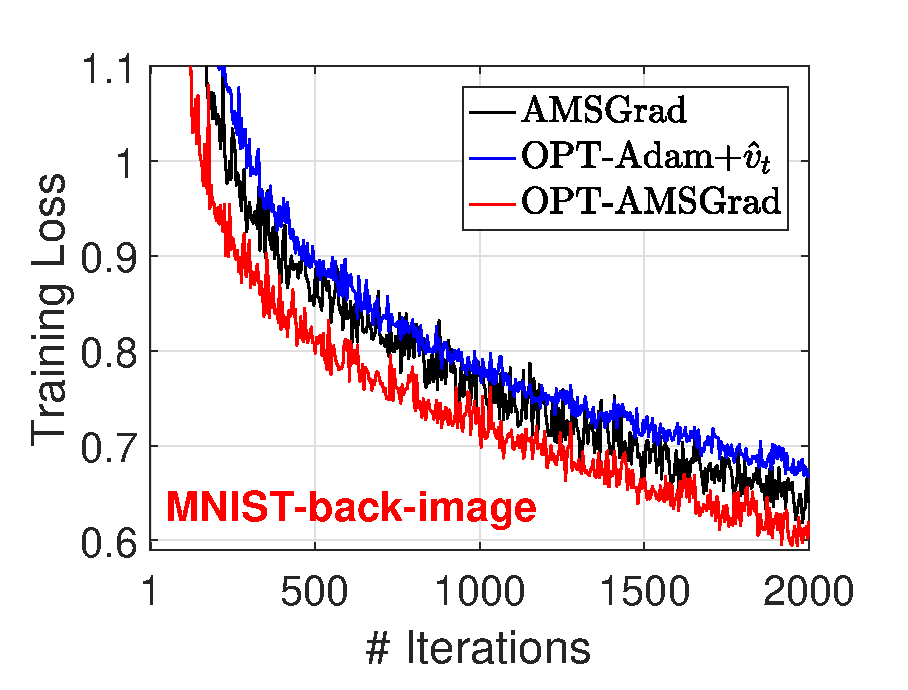
\includegraphics[width=1.45in]{simulation/fig2/M_image_train_loss_no1.eps}
}
\quad
\subfigure{
\includegraphics[width=1.45in]{simulation/fig2/cifar_cnn_train_loss_no1.eps}
}
}
\vspace{-0.1in}
\mbox{
\subfigure{
\includegraphics[width=1.45in]{simulation/fig2/imdb_lstm_train_loss_no1.eps}
}
\quad
\subfigure{
\includegraphics[width=1.45in]{simulation/fig2/cifar10_resnet_train_loss.eps}
}
\quad
\subfigure{
\includegraphics[width=1.45in]{simulation/fig2/cifar100_resnet_train_loss.eps}
}
}
\caption{Training loss vs. Number of iterations. The first row are results with fully-connected neural network.}
\label{train_loss}
\end{figure}


We are also curious about the long-term performance and generalization of the proposed method in test phase. In Figure~\ref{figs:M_image_new3}, Figure~\ref{figs:CIFAR10_new3} and Figure~\ref{figs:CIFAR100_new3}, we plot the corresponding results when the model is trained to the state with stable test accuracy. We observe: 1) In the long term, \textsc{OPTIMISTIC-AMSGrad} algorithm may converge to a better point with smaller objective function value, and 2) In this three applications, the proposed \textsc{OPTIMISTIC-AMSGrad} also outperforms the competing methods in terms of test accuracy. These are also important benefits of \textsc{OPTIMISTIC-AMSGrad}.

\begin{figure}[H]
\centering
\mbox{
\subfigure{
\includegraphics[width=1.30in]{./new_figure/new_mnist_img_figure/mnist_img_train_loss_disz_2.eps}\hspace{-0.1in}
}
\quad
\subfigure{
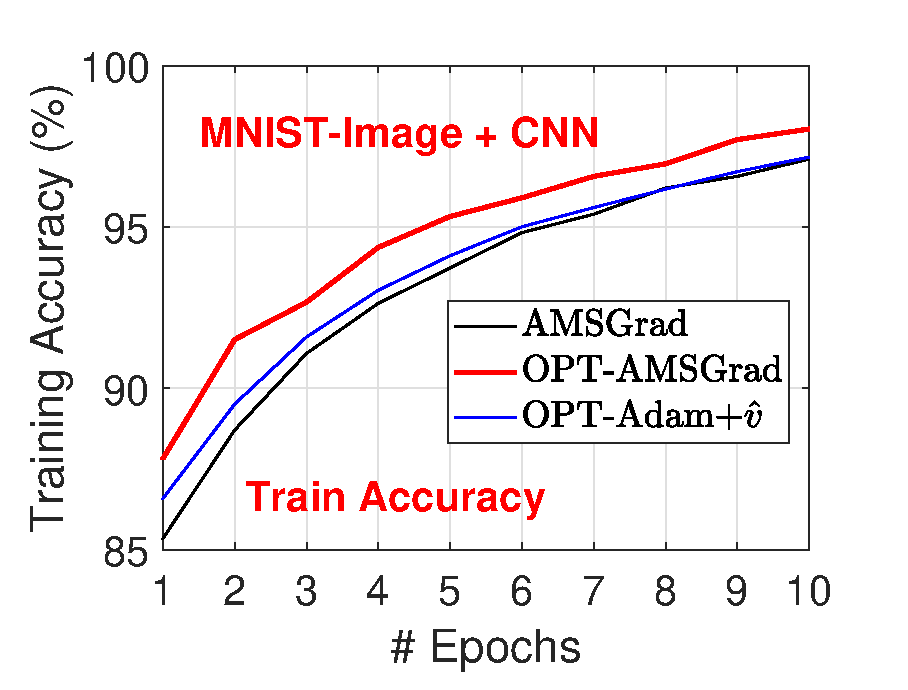
\includegraphics[width=1.30in]{./new_figure/new_mnist_img_figure/mnist_img_train_acc_disz_2.eps}\hspace{-0.1in}
}
\quad
\subfigure{
\includegraphics[width=1.30in]{./new_figure/mnist_img_test_loss_disz.eps}\hspace{-0.1in}
}
\subfigure{
\includegraphics[width=1.30in]{./new_figure/mnist_img_test_acc_disz.eps}
}
}

\mbox{
\subfigure{
\includegraphics[width=1.30in]{./new_figure/cifar10_train_loss_disz.eps}\hspace{-0.1in}
}
\quad
\subfigure{
\includegraphics[width=1.30in]{./new_figure/cifar10_train_acc_disz.eps}\hspace{-0.1in}
}
\quad
\subfigure{
\includegraphics[width=1.30in]{./new_figure/cifar10_test_loss_disz.eps}\hspace{-0.1in}
}
\subfigure{
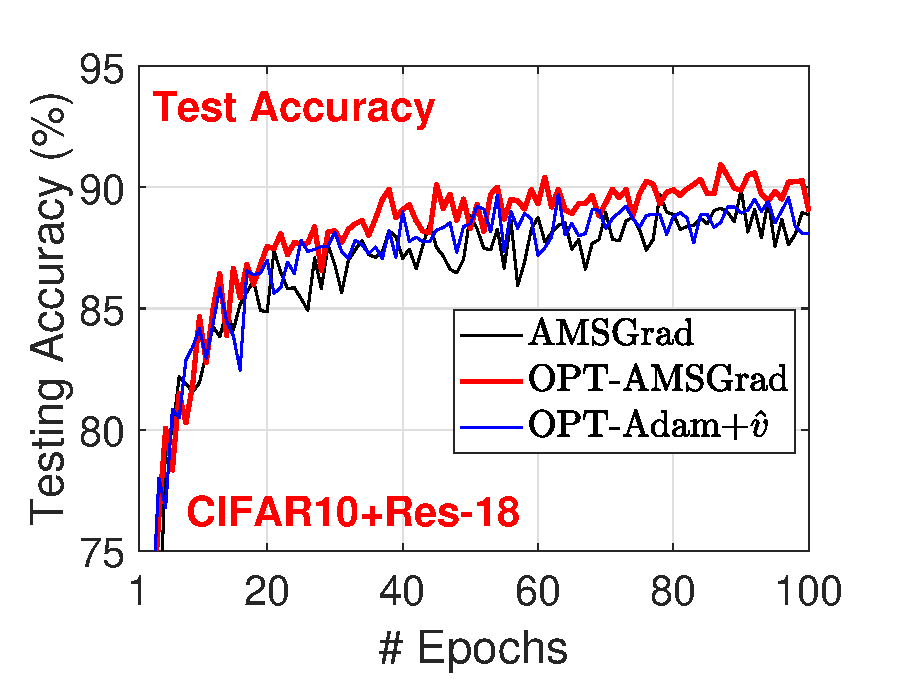
\includegraphics[width=1.30in]{./new_figure/cifar10_test_acc_disz.eps}
}
}
\mbox{
\subfigure{
\includegraphics[width=1.30in]{new_figure/cifar100_train_loss_disz.eps}\hspace{-0.1in}
}
\quad
\subfigure{
\includegraphics[width=1.30in]{new_figure/cifar100_train_acc_disz.eps}\hspace{-0.1in}
}
\quad
\subfigure{
\includegraphics[width=1.30in]{new_figure/cifar100_test_loss_disz.eps}\hspace{-0.1in}
}
\subfigure{
\includegraphics[width=1.30in]{new_figure/cifar100_test_acc_disz.eps}
}
}
\caption{\textit{MNIST-back-image} + CNN, \textit{CIFAR10} + Res-18 and \textit{CIFAR100} + Res-50 . We compare three methods in terms of training (cross-entropy) loss, training accuracy, testing loss, and testing accuracy. We observe that \textsc{Optimistic-AMSGrad} consistently improves the two baselines.} \label{figs:CIFAR10_new3}
\end{figure}

\subsection{Choice of parameter $r$}
Recall that our proposed algorithm has the parameter $r$ that governs the use of past information.
Figure~\ref{fig:compare-r} compares the performance under different values of $r=3,5,10$ on two datasets. From the result we see that the choice of $r$ does not have significant impact on learning performance. Taking into consideration both quality of gradient prediction and computational cost, it appears that $r=5$ is a good choice. We remark that empirically, the performance comparison among $r=3,5,10$ is not absolutely consistent (i.e. more means better) in all cases. One possible reason is that for deep neural nets which have very complicated and highly non-convex landscape, using gradient information from too long ago may not be helpful in accurate gradient prediction. Nevertheless, $r=5$ seems to be good for most applications.

\begin{figure}[H]
\begin{center}
\mbox{
\includegraphics[width=1.65in]{./new_figure/new_mnist_img_figure/mnist_img_train_loss_r3510_2.eps}\hspace{-0.1in}
\includegraphics[width=1.65in]{./new_figure/cifar10_train_loss_r3510.eps}
}
\end{center}
\vspace{-0.1in}
\caption{The training loss of \textsc{OPTIMISTIC-AMSGrad} with different $r$.}     \label{fig:compare-r}
\end{figure}


\section{Concluding Remarks}
\subsection{Discussion on the iteration cost}

We observe that the iteration cost (i.e., actual running time per iteration) of our implementation of \textsc{Optimistic-AMSGrad} with $r=5$ is roughly two times larger than the standard \textsc{AMSGrad}. When $r=3$, the cost is roughly 0.7 times longer. Nevertheless, \textsc{OPTIMISTIC-AMSGrad} may still be beneficial in terms of training efficiency, since fewer iterations are typically needed. For example, in Figure \ref{figs:CIFAR10_new3} and \ref{figs:CIFAR100_new3}, to reach the training loss of \textsc{AMSGrad} at 100 epochs, the proposed method only needs roughly 20 and 40 epochs, respectively. That said, \textsc{OPTIMISTIC-AMSGrad} needs 40\% and 80\% time to achieve same training loss as \textsf{AMSGrad}, in this two problems.

The computational overhead mostly comes from the gradient extrapolation step. More specifically, recall that the extrapolation step consists of:
(a) The step of constructing the linear system $(U^\top U)$.
The cost of this step can be optimized and reduced to $\mathcal O(d)$, since the matrix $U$ only changes one column at a time.
(b) The step of solving the linear system.
The cost of this step is $O(r^3)$, which is negligible as the linear system is very small ($5$-by-$5$ if $r=5$).
(c) The step that outputs an estimated gradient as a weighted average of previous gradients.
The cost of this step is $\mathcal O(r \times d)$. Thus, the computational overhead is $\mathcal O\left((r+1)d+r^3\right)$.
Yet, we notice that step (a) and (c) is parallelizable, so they can be accelerated in practice.

\noindent \textbf{Memory usage:} Our algorithm needs a storage of past $r$ gradients for each coordinate, in addition to the estimated second moments and the moving average. Though it seems demanding compared to the standard AMSGrad, it is relatively cheap compared to Natural gradient method (e.g.,~\cite{MG15}), as Natural gradient method needs to store some matrix inverse.

\subsection{Conclusion}
In this paper, we propose \textsc{Optimistic-AMSGrad}, which combines optimistic learning and \textsc{AMSGrad} to improve sampling efficiency and
accelerate the process of training, in particular for deep neural networks. With a good gradient prediction, the regret can be smaller than that of standard \textsc{AMSGrad}. Experiments on various deep learning problems demonstrate the effectiveness of the proposed method in improving the training efficiency. 

\bibliography{reference}
\bibliographystyle{plain}



\end{document}